\documentclass{article}
\usepackage{float}
\usepackage{amsmath,amssymb,amsthm,graphicx}
\usepackage{subcaption}
\usepackage{mleftright}
\usepackage{tikz}
\usepackage{tikz-network}


\setlength{\oddsidemargin}{0.25 in}
\setlength{\evensidemargin}{-0.25 in}
\setlength{\topmargin}{-0.6 in}
\setlength{\textwidth}{6.5 in}
\setlength{\textheight}{8.5 in}
\setlength{\headsep}{0.75 in}
\setlength{\parindent}{0 in}
\setlength{\parskip}{0.1 in}

\newtheorem{theorem}{Theorem}
\newtheorem{corollary}{Corollary}
\newtheorem{proposition}{Proposition}
\newtheorem*{remark}{Remark}
\theoremstyle{definition}
\newtheorem{example}{Example}
\newtheorem{definition}{Definition}

\newcommand{\lecture}[4]{
   \pagestyle{myheadings}
   \thispagestyle{plain}
   \newpage
%   \setcounter{lecnum}{#1}
   \setcounter{page}{1}
   \noindent
   \begin{center}
   \framebox{
      \vbox{\vspace{2mm}
    \hbox to 6.58in { {\bf CSC~565: Graph Theory
                        \hfill North Carolina State University} }
    \hbox to 6.58in { {\bf Fall 2019
                        \hfill Computer Science} }
       \vspace{4mm}
       \hbox to 6.28in { {\Large \hfill Lecture #1: #2  \hfill} }
       \vspace{2mm}
       \hbox to 6.28in { {\it Lecturer: {\it Don Sheehy {\tt <drsheehy@ncsu.edu>}} \hfill Scribe: #4} }
      \vspace{2mm}}
   }
   \end{center}
   \markboth{Lecture #1: #2}{Lecture #1: #2}
   \vspace*{4mm}
}


\begin{document}
%FILL IN THE RIGHT INFO.
%\lecture{**LECTURE-NUMBER**}{**DATE**}{**LECTURER**}{**SCRIBE**}
\lecture{28}{Dec 2, 2019}{Hongyi Fan, Guangyu Yu Scribe}
%\footnotetext{These notes are partially based on those of Nigel Mansell.}

% **** YOUR NOTES GO HERE:

% Some general latex examples and examples making use of the
% macros follow.  
%**** IN GENERAL, BE BRIEF AND COMPLETE. 

\section{Decision problems} 

Decision problems:
input: number
output: accept/reject

Not all decision problems are decidable.
    \begin{figure}[h!]
		\begin{center}
			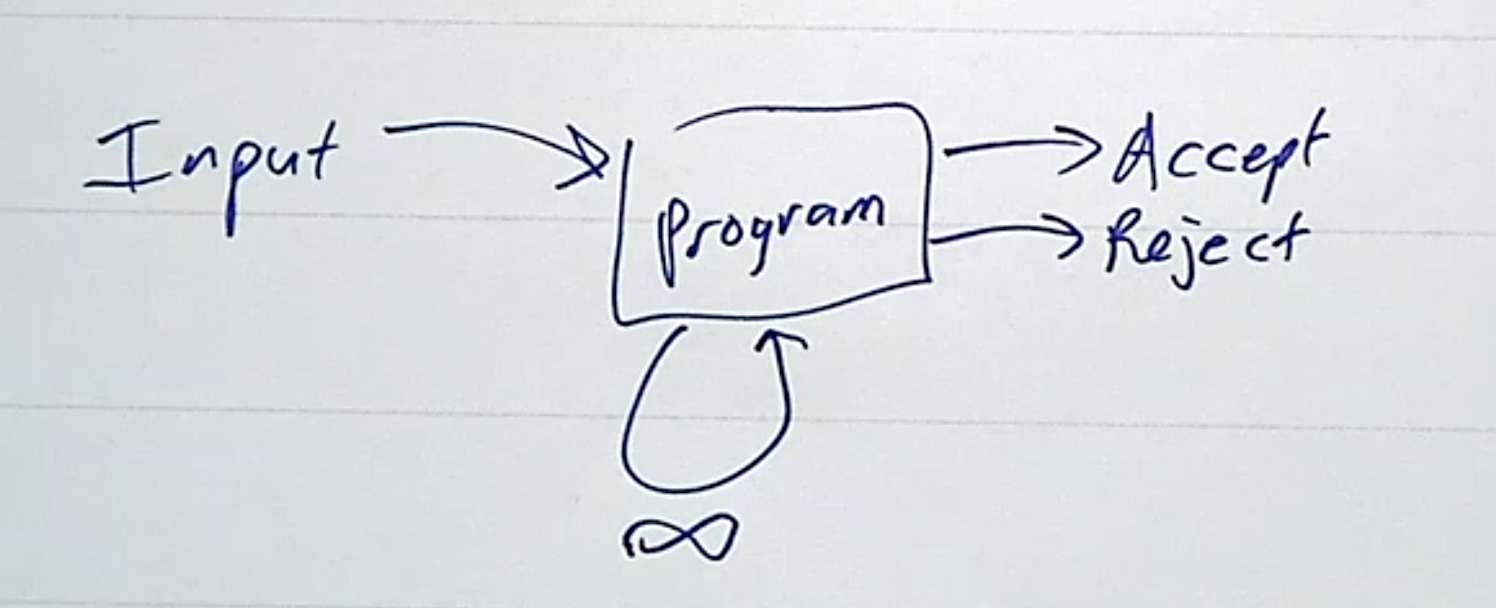
\includegraphics[scale=0.3]{images/fig1}
		\end{center}
		\caption{Decision problem}
	\end{figure}
Halting problem is the problem of determining, from a description of an arbitrary computer program and an input, whether the program will finish running, or continue to run forever.
Programs are stored as data, or string of bits, or just number.

Cantor's Diagonalization: a mathematical proof that there are infinite sets which cannot be put into one-to-one correspondence with the infinite set of natural numbers.
    \begin{figure}[h!]
		\begin{center}
			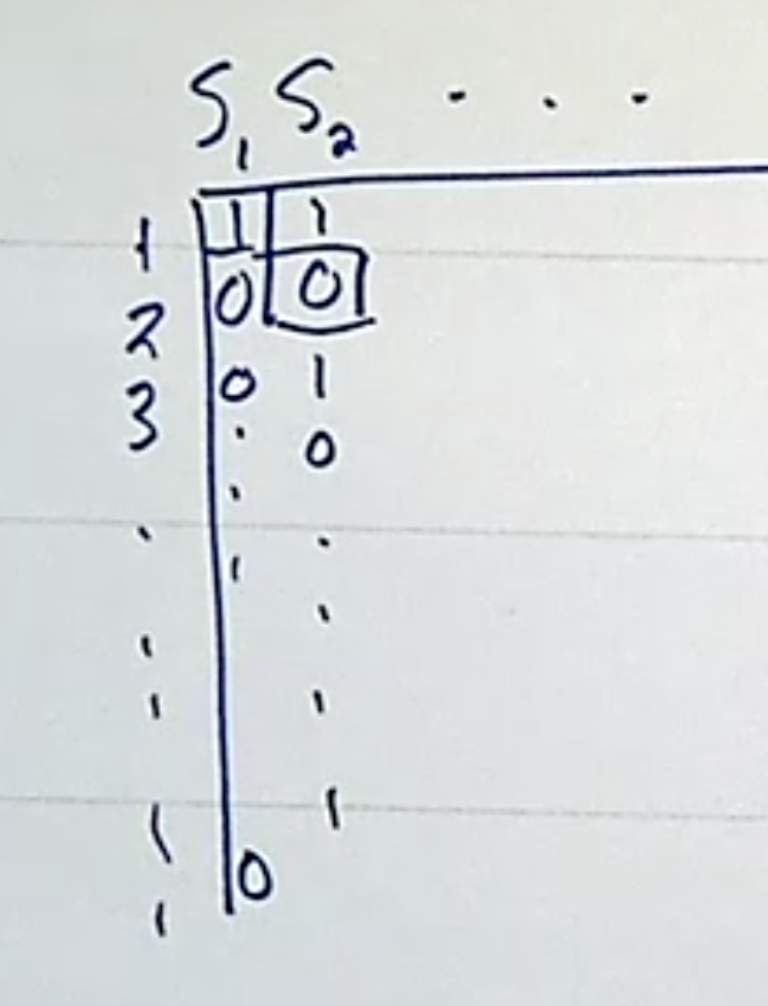
\includegraphics[scale=0.3]{images/fig2}
		\end{center}
		\caption{Cantor's Diagonalization}
	\end{figure}
	
$S_*$ = \{i: i\nsubseteq$S_i$\} \\
Suppose  $S_*$ = $S_i$ for some i \\
i\subseteq $S_*$ iff i\nsubseteq $S_*$ \Rightarrow \perp\\\\

Diagonal Language: D = \{P$|$P($<$P$>$) does not accept \}\\
\begin{theorem}
D is undecidable.
\end{theorem}
\begin{proof}
Suppose D is decidable.\\
Let Q be a program that decides D.\\
Q \in D?\\
if\ Q(<Q>)$ accepts then Q $\notin D\\
if\ Q(<Q>)$ rejects then Q $\in D
\end{proof}

Reduction\\
A reduces to B: A is not harder than B, so we can use a solution to B to solve A.\\
Suppose A is impossible then B is impossible.\\\\


Halt = \{$<P, w>|P(w)\ halts$ \}
\begin{theorem}
halt is undecidable.
\end{theorem}
\begin{proof}
Suppose Q decides halt.\\
program: R(P):\\Run Q(P, $<$P$>$)\\if it accepts run p($<$P$>$) and return opposite of P($<$P$>$)\\Else reject\\
R decides Diag. \Rightarrow \perp
\end{proof}

\section{A problem with graph}
Goal: construct a space X \subseteq $R^2$ \\s.t. The problem $Embed_X$ = \{G: G is a graph that can be embeded in X \} is undecidable.

U: undecidable problem as a set of numbers.\\
X = \underset{n \in U}{\cup}geom($G_n$)\\
Reduction: instances(a number n) to graphs($G_n$: $C_n$ + triangles on edges)\\
Claim: $G_n$ embeds into X iff n \in U\\$G_n$ \in $Embed_x$
    \begin{figure}[h!]
		\begin{center}
			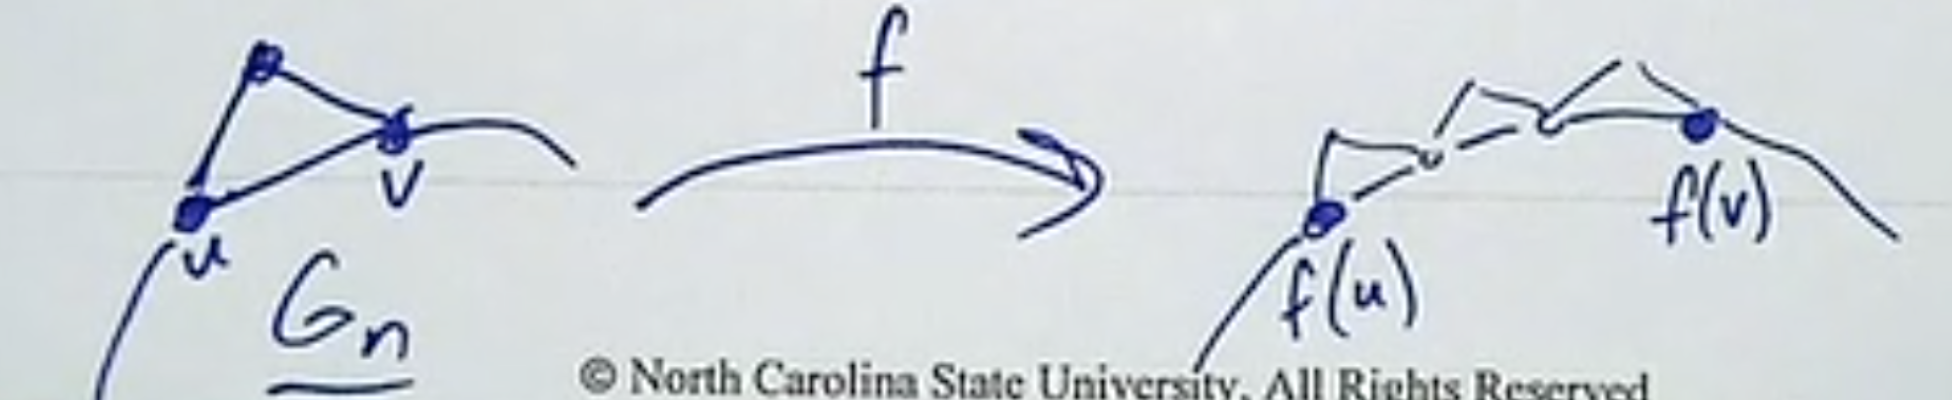
\includegraphics[scale=0.3]{images/fig3}
		\end{center}
	\end{figure}
\begin{proof}
$G_n$\hookrightarrow$G_m$ \implies m=n\\
{\bf if}\ m < n $ then there is no place for all n deg 4 vertices to map to.$\\
{\bf if}\ m > n $ then 2 adjacent vertices in $G_n$ are not adjacent in $G_m$.$\\
{\bf if}\ $G_n$\hookrightarrow X \ {\bf then}\ n \in U \ because f($G_n$) is in some connected component of X.\\
so f($G_n$) \subseteq $G_m$ \implies m = n.\\
cr(G) = $min number of crossings for any embedding of G into the plane.$\\
m \leq 3n-6 $ for planar graphs$ \\
cr(G) \geq m-3n+6\\
G=(V, E) |V|=n, |E|=m\\
H \subseteq G, $V_H$ is formed by removing each vertex of g with probability of 1-p\\
E(|$V_H$|)=pn E(|$E_H$|)=$p^2$m\\
E(cr(H)) \leq $p^4$cr(G) $m^3$=$n^4$\\
so cr(G) \geq $n^2$/64
\end{proof}

\end{document}

